\documentclass{beamer}
\usetheme{Boadilla}
\usepackage{tikz}
\usetikzlibrary{shapes.geometric, arrows}
\documentclass{article}
\usepackage{graphicx}
\graphicspath{ {./images/} }

\title{Route Optimization Algorithm}
\author{Indian Institute of Technology, Bombay }
\date{\today}
\tikzstyle{startstop} = [rectangle, rounded corners, minimum width=2cm, minimum height=1cm,text centered, draw=black]
\tikzstyle{arrow} = [thick,->,>=stealth]


\begin{document}

\begin{frame}
\begin{titlepage}
\begin{center}
    \includegraphics[width=2.9cm]{iitb.png}
\end{center}
\end{titlepage}
\end{frame}

\begin{frame}{The Problem}
\begin{itemize}
\item Single Depot Vehicle Scheduling Problem
\item It is a combinatorial optimization problem for which finding the optimal solution is NP hard. Hence generally heuristic approaches are taken according to the size of data
\item Constraints:
\begin{itemize}
    \item Time window
    \item Bus capacity; limit and minimum 85\% occupancy
    \item Number of buses
\end{itemize}
\item The objective is to minimise the operational cost of buses
\end{itemize}
\end{frame}

\begin{frame}{Impact of the Problem}
\begin{itemize}[<+- | alert@+>]
\item The problem is important to be addressed because of its evident commercial and economical impact
\item Owing to the large scale at which buses are used, even a 5\% improvement can significantly reduce the carbon footprint
\item Solving this problem also helps in issues like Garbage Truck Scheduling and Goods Delivery Scheduling
\item This problem is generally approached using Integer Programming, by forming a set of equations and finding solutions and optimizing the process by using methods like ant colonization
\end{itemize}
\end{frame}

\begin{frame}{Flow of Solving}
\begin{center}
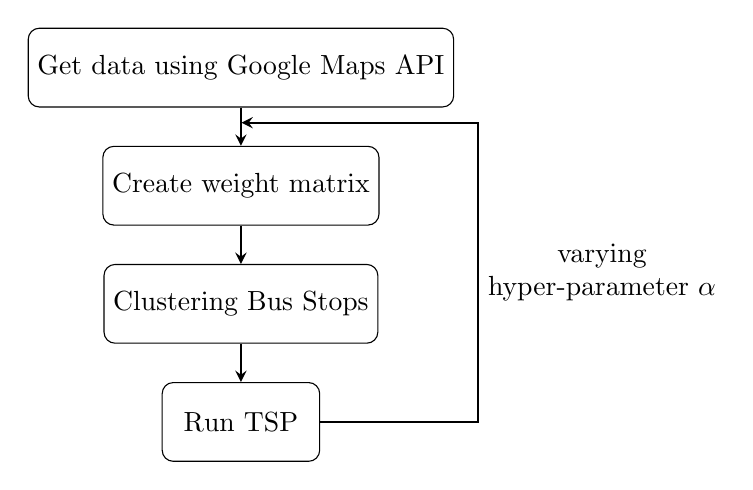
\begin{tikzpicture}[node distance=1.5cm]
\node (step1) [startstop] {Get data using Google Maps API};
\node (step2) [startstop, below of=step1] {Create weight matrix};
\node (step3) [startstop, below of=step2] {Clustering Bus Stops};
\node (step4) [startstop, below of=step3] {Run TSP};
\draw [arrow] (step1) -- (step2);
\draw [arrow] (step2) -- (step3);
\draw [arrow] (step3) -- (step4);
\draw [arrow] (step4.east) -- ++(2.0cm,0)
 |- node[right, pos=0.25,align=center]{varying \\ hyper-parameter $\alpha$} ++(0,3.8cm) -- ++(-3.0cm,0);
\end{tikzpicture}
\end{center}
\end{frame}
\begin{frame}{Travelling Salesman Problem(TSP)}

\begin{itemize}[<+- | alert@+>]

\item What is TSP and why TSP?
\item Since its time complexity is O($n^2$ $2^n$), we cannot use the algorithm directly as it is very inefficient
\item We use clustering on the bus stops to improve the overall time complexity
\item Once the bus stops are in clusters we will assign one bus to each cluster and use TSP to determine route of the bus

\end{itemize}
\centering
\includegraphics[width=3.5cm]{bosch_img1.jpg}
\end{frame}


\begin{frame}{Why clustering improves time}
\begin{itemize}[<+- | alert@+>]
\item Assume ‘n’ nodes (bus stops)
\item If the n nodes are divided in k clusters, with $n_i$
nodes in each cluster, such that
$n_i$ \approx  $ n_j$ for all i,j, thus $kn_i = n$
Time complexity for TSP for each cluster is O($n_i^2$ $2^{n_i}$)
\item Thus,  $T_{without clustering} \propto n^2 2^n$ and $T_{with clustering} \propto kn_i^2 2^{n_i}$
Therefore,  \[ \frac{T_{without clustering}}{T_{with clustering}} = {k.2^{n(1-1/k)}}    \]
\item For a fixed n, $T_{without clustering}$ is constant. As number of clusters k increases, ${k.2^{n(1-1/k)}}$ increases exponentially, thus $T_{with clustering}$ decreases
\item Hence with increase in number of clusters k, the time taken for TSP decreases exponentially 

\end{itemize}
\end{frame}

\begin{frame}{Clustering}
\begin{itemize}[<+- | alert@+>]
\item K-Means clustering has been used
\item Since each bus is going to cover all bus stops in a cluster, the number of stops in each cluster must satisfy the size constraints of the bus
\item Number of clusters should not exceed the number of buses available
\item For number of clusters $k$, we find the smallest integer $k$ satisfying:
\[ k> \text{(number of people)} / \text{(bus capacity)}\]

\item If the size of a cluster exceeds bus capacity then treat this cluster as an independent problem and use the procedure recursively over it
\end{itemize}
\end{frame}
\begin{frame}{Clustering of the newly given data}
\includegraphics[width=\textwidth]{clustering_image.png}
\end{frame}


\begin{frame}{Handling the Time Window constraint}
\begin{itemize}[<+- | alert@+>]
\item The TSP used previously considered only distances between the stops and not time
\item We replace the distances with a weighted average of distance between the stops and the time required to go from one stop to the other
\[ weight(i,j) = \alpha \times distance(i,j) + (1-\alpha) \times time(i,j) \times v\]
Where v = average speed of the bus
\item Run the TSP using these weights for a range of values of $\alpha$
\item $\alpha$ = 1 will give the minimum distance solution ignoring time window, $\alpha$ = 0 will give the minimum time solution ignoring cost
\item We want to have a solution such that the time taken by the buses falls within the time window. We will use a particular value for $\alpha$
\end{itemize}
\end{frame}
\begin{frame}{Handling the Time Window constraint}
\begin{center}
\includegraphics[width=0.45\textwidth]{time_w_bid.png}

\includegraphics[width=0.45\textwidth]{time_wo_bid.png}
\end{center}

\end{frame}
\begin{frame}{Handling the Distance constraint}
\begin{center}
\includegraphics[width=0.45\textwidth]{dist_w_bid.png}
\includegraphics[width=0.45\textwidth]{dist_wo_bid.png}
\end{center}
\end{frame}

% \begin{frame}{Time taken by buses vs. $\alpha$}
% GRAPH
% \end{frame}

\begin{frame}{Handling Real Time Traffic}
\begin{itemize}[<+- | alert@+>]
\item Mark the points which have been covered as visited
\item Schedule a Cron job for every 15 mins(say) which makes API calls to get distance and time matrix for only those points which are unvisited and update the weight matrix
\item Clustering remains same
\item For each cluster find path of minimum weight covering all nodes where begin and end points are not the same
\item This is solved in the way same as that for TSP with a modified equation for Dynamic Programming
\item The time for this computation will be lesser than that of the TSP done initially as number of points have reduced and hence also efficient
\end{itemize}
\end{frame}

\begin{frame}{Results}
\begin{itemize}[<+- | alert@+>]
\item In the given data set, the number of people boarding is 95
\item Since bus capacity is 50 and number of people 95, it is optimum to use 2 buses, 1 bus doesn't work, more than 2 buses will lead to atleast one bus with occupancy less than 85\%
\item An optimal solution is to use 2 buses following the routes :

\end{itemize}
\end{frame}

\begin{frame}{Results}
\includegraphics[width=0.9\textwidth]{bus_routes.png}
\end{frame}


\begin{frame}{Results}
\begin{itemize}
\item For the given sample data set, no solution is possible which satisfies all the given constraints
\item Reason is that the depot 'Bosch Bidadi' is itself at a far off distance from the other stops, explained on maps
\item 'Mantri Apartment' is itself 50 km and at a time of 1 hr from the depot, while time window is of 1hr 20 min
\item We can handle such outliers
\item Since number of people is 29 and 85\% of bus capacity is 27, only one bus can be used. Solution for this leads to a minimum time of \b{4 hrs} which is not acceptable
\item Possible way to reduce time is to use 2 or more buses but then they will have less occupancy

\end{itemize}
\end{frame}

\begin{frame}{Results}
    \includegraphics[width=\textwidth]{screen.png}
\end{frame}

\begin{frame}{Challenges faced}
\begin{itemize}[<+- | alert@+>]
    \item While using Google Maps APIs to get distances and travel time between places, some places were causing ambiguities, eg. for Jantha Bazar, the location being returned was over $1000$km from Bosch Bidadi
    \item To handle this, whenever there are such locations which have an average distance more than 100 km from the other points, we append the city name to it for the API call
\end{itemize}
\end{frame}
\begin{frame}{Quantum Algorithm to solve the TSP}
\begin{itemize}[<+- |alert@+>]
    \item NP hard problem in combinatorial optimization takes exponential time order for solving by classical brute force method
    \item Quantum Algorithm solves the TSP using phase estimation technique. Distance between points is encoded as phases
    \item Construct unitary operators whose eigenvectors are the computational basis states and eigenvalues are various combinations of these phases
    \item Then we apply phase estimation algorithm to certain eigenstates which give us all the total distances possible for all the routes
    \item After obtaining the distances we can search through this information using the quantum search algorithm for finding the minimum to find the least possible distance as well the route taken
    \item This provides us a quadratic speedup over the classical brute force method for a large number of cities
    \footnote{\textit{Karthik Srinivasan, Saipriya Satyajit, Bikash K Behera, and Prasanta K. Panigrahi}, \textbf{Efficient quantum algorithm for solving travelling salesman problem: An IBM quantum experience}}
\end{itemize}

\end{frame}
\end{document}
